\documentclass[12pt]{amsart}
% Default margins are too wide all the way around. I reset them here
\setlength{\hoffset}{-.75in}
\setlength{\textwidth}{6.5in}
\setlength{\voffset}{-.5in}
\setlength{\textheight}{9.0in}
\usepackage{amsmath}
\usepackage{amssymb}
\usepackage{amsthm}
\usepackage{pgfplots}
\usepackage{enumerate}
\usepackage{tikz}
\usetikzlibrary{shadows,arrows,arrows.meta,shapes,positioning,calc}% Required for the Circle and Triangle arrow tips
\usepackage{setspace}
\usepackage{siunitx}
\usepackage{enumitem}
\usepackage{tcolorbox}
\usepackage{array}
\usepackage{microtype}
\usepackage{hyperref}


\theoremstyle{conjecture}
\newtheorem{conjecture}{Conjecture}

\theoremstyle{definition}
\newtheorem{definition}{Definition}

\theoremstyle{question}
\newtheorem{question}{Question}

\theoremstyle{theorem}
\newtheorem{theorem}{Theorem}

\newenvironment{solution}
{\begin{proof}[Solution]}
{\end{proof}}

\newcommand{\sectionrule}{%
    \vspace{0.3em}
    \hrule
    \vspace{0.8em}
}

\newcommand{\phaseplot}[1]{%
    \par\medskip
    \noindent\begin{minipage}{\linewidth}
    \centering
    \begin{tikzpicture}
    \begin{axis}[
    width=0.61\linewidth,height=4.75cm,
    axis lines=middle,
    xmin=-3.3,xmax=3.3,ymin=-1.12,ymax=1.16,
    xtick={-3,-2,-1,1,2,3},ytick={-1,-0.5,0.5,1},
    minor tick num=4,
    xlabel={$x$},ylabel={},
    title={\small functions},title style={yshift=-0.6em},
    tick label style={font=\small},
    every axis x label/.style={at={(ticklabel* cs:1)},anchor=west},
    axis line style={gray!70},tick style={gray!70},
    clip=false]
    \addplot[blue!55!gray,thick,domain=-3.3:3.3,samples=150]{sin(deg(x))};
    \addplot[orange!85!yellow!70!black,thick,domain=-3.2:3.2]{#1};
    \end{axis}
    \end{tikzpicture}
    \end{minipage}
    \par\medskip}

\title{Dynamical Systems:\\Class September 3, 2026\\ 4. Flow on the Circle.}
\author{Rob Tompkins}
\date{\today}


\begin{document}

    \maketitle
    \section*{Skill Check practice}
    \begin{enumerate}
        \item Assume the time evolution of the phase difference, $\phi$, between an oscillator and a reference
        signal is given by the system $\dot\phi=1.1-\sin\phi$.

        \phaseplot{1.1}

        What is the long term behavior of the phase difference in this system? \emph{If it approaches a fixed
        value, provide an estimate of that value.}

        Extra example: $\dot\phi=0.8-\sin\phi$

        \phaseplot{0.8}

        \item Draw the phase portrait for a 1D differential equation both on the real line and also on the
        circle.
    \end{enumerate}

    \section*{Skill Check practice solution}
    \textbf{Answer:} the phase difference is drifting (always increasing).

    \textbf{Explanation} (not needed on the skill check itself):

    \hspace*{1.5em}This question requires us to interpret $\phi$ as a phase difference, rather than as the phase of a single
    oscillator.

    \newpage

    \hspace*{1.5em}If there were an intersection between the sinusoid and the straight line then the phase difference
    would approach a fixed value (that you could identify) associated with a stable or half-stable fixed
    point.

    \hspace*{1.5em}In this picture, though, $\dot\phi=1.1-\sin\phi$ and $\sin\phi<1.1$ for all values of $\phi$. So
    $\dot\phi>0$ for all phase differences, $\phi$. This means that the \textbf{phase difference is always
    changing}. In some sense, it is always increasing ($\dot\phi>0$, after all). However, when the phase
    difference passes through $2\pi n$ for $n$ an integer, the oscillator and the reference momentarily
    have the same phase angle, so if we look at the two oscillators on a circle, one of them will appear to
    `lap' the other one over and over again.

    \section*{Period of the oscillation: see section 4.3}
    \hspace*{1.5em}Consider the system $\dot\theta=\omega-a\sin\theta$. Integrate the time over one oscillation period $T$:
    \[
        T=\int_0^T dt
        =\int_0^{2\pi}\frac{dt}{d\theta}\,d\theta
        =\int_0^{2\pi}\frac{1}{\omega-a\sin\theta}\,d\theta
    \]

    \hspace*{1.5em}Here we first made a change of variables in the integration from $t$ to $\theta$, and then noted that
    $dt/d\theta=1/\dot\theta$.

    \section*{}
    \newpage

    \section*{Teams}
    Post screenshots of your work to the course Google Drive today:\href{https://drive.google.com/}{Link to drive folder}.
    Include words, labels, and other short notes on your whiteboard that might make those solutions useful
    to you or your classmates. Name your images using the format:

    \begin{itemize}
        \item \texttt{teamXX-YY.EXT}
    \end{itemize}

    where XX is your two-digit team number (e.g. 06 if you are team 6), YY is the two digit number of image
    for today (e.g. 01 for the first image, 02 for the second, and so on.), and EXT is the extension for the
    image filetype you used.

    \section*{Team Activity}
    \begin{enumerate}
        \item (4.1.1) For which values of $a$ does the equation $\dot\theta=\sin(a\theta)$ give a well-defined
        vector field on the circle? Recall that, in order to be well defined on the circle, the flow must repeat
        itself as you make a full revolution around the circle.

        For $a=3$, find and classify all the fixed points and sketch the phase portrait on the circle. It may
        help to make a plot of $\sin(3\theta)$.

        \begin{solution}
            For the vector field to be well-defined on the circle, it must be
            $2\pi$-periodic:
            \[
                \sin\bigl(a(\theta+2\pi)\bigr)=\sin(a\theta)
                \qquad\text{for every }\theta.
            \]
            Using the angle-addition formula,
            \[
                \sin(a\theta+2\pi a)
                =\sin(a\theta)\cos(2\pi a)
                +\cos(a\theta)\sin(2\pi a).
            \]
            This equals $\sin(a\theta)$ for every $\theta$ precisely when
            \[
                \cos(2\pi a)=1
                \qquad\text{and}\qquad
                \sin(2\pi a)=0.
            \]
            Therefore,
            \[
                \boxed{a\in\mathbb{Z}}.
            \]

            For $a=3$, the fixed points satisfy
            \[
                \sin(3\theta)=0,
            \]
            and hence, modulo $2\pi$,
            \[
                \theta=0,\ \frac{\pi}{3},\ \frac{2\pi}{3},\
                \pi,\ \frac{4\pi}{3},\ \frac{5\pi}{3}.
            \]
            Let $f(\theta)=\sin(3\theta)$. Since
            \[
                f'(\theta)=3\cos(3\theta),
                \qquad
                f'\left(\frac{k\pi}{3}\right)=3(-1)^k,
            \]
            the fixed points with even $k$ are unstable, while those with odd
            $k$ are stable. Thus
            \[
                \boxed{
                    \begin{aligned}
                        \text{unstable:}\quad&0,\ \frac{2\pi}{3},\ \frac{4\pi}{3},\\
                        \text{stable:}\quad&\frac{\pi}{3},\ \pi,\ \frac{5\pi}{3}.
                    \end{aligned}}
            \]
            The arrows point away from each open (unstable) point and toward the
            neighboring filled (stable) points:

            \begin{center}
                \begin{tikzpicture}[scale=1.75,>=Stealth]
                  \def\r{1}
                  \draw[thick] (0,0) circle (\r);

                  % Direction of the flow on each arc.
                  \draw[->,thick] ({\r*cos(15)},{\r*sin(15)})
                  arc[start angle=15,end angle=43,radius=\r];
                  \draw[->,thick] ({\r*cos(105)},{\r*sin(105)})
                  arc[start angle=105,end angle=77,radius=\r];
                  \draw[->,thick] ({\r*cos(135)},{\r*sin(135)})
                  arc[start angle=135,end angle=163,radius=\r];
                  \draw[->,thick] ({\r*cos(225)},{\r*sin(225)})
                  arc[start angle=225,end angle=197,radius=\r];
                  \draw[->,thick] ({\r*cos(255)},{\r*sin(255)})
                  arc[start angle=255,end angle=283,radius=\r];
                  \draw[->,thick] ({\r*cos(345)},{\r*sin(345)})
                  arc[start angle=345,end angle=317,radius=\r];

                  % Unstable fixed points (open circles).
                  \foreach \angle/\label in {
                      0/{0},
                      120/{\frac{2\pi}{3}},
                      240/{\frac{4\pi}{3}}
                  }{
                      \draw[thick,fill=white]
                      ({\r*cos(\angle)},{\r*sin(\angle)}) circle (1.7pt);

                      \node at
                      ({1.28*\r*cos(\angle)},{1.28*\r*sin(\angle)})
                          {$\label$};
                  }

                  % Stable fixed points (filled circles).
                  \foreach \angle/\label in {
                      60/{\frac{\pi}{3}},
                      180/{\pi},
                      300/{\frac{5\pi}{3}}
                  }{
                      \fill
                      ({\r*cos(\angle)},{\r*sin(\angle)}) circle (1.9pt);

                      \node at
                      ({1.28*\r*cos(\angle)},{1.28*\r*sin(\angle)})
                          {$\label$};
                  }
                \end{tikzpicture}
            \end{center}
        \end{solution}

        \item (4.3.3) For $\dot\phi=\mu\sin\phi-\sin 2\phi$:
        \begin{enumerate}[label=(\alph*),leftmargin=2.6em,itemsep=0.3em]
          \item Check that the vector field is well-defined on the circle
          \item Draw phase portraits for:
          \begin{itemize}
              \item large positive $\mu$
              \item $\mu=0$
              \item large negative $\mu$
          \end{itemize}
          \item Use $\sin 2\phi=2\cos\phi\sin\phi$ to find mathematical expressions for fixed points.
          \item Classify the bifurcations that occur as $\mu$ varies.
          \item Find the bifurcation values of $\mu$.
          \item Think of $\phi$ as describing the \textbf{phase of a single oscillator}. For what values of
          $\mu$ is the system ``oscillating''?
          \item Think of $\phi$ as describing the \textbf{phase difference} between an oscillator and a
          reference. For what values of $\mu$ is the oscillator entrained (phase-locked) to the reference?
          What sets their phase difference?
        \end{enumerate}

        \begin{solution}
            Write
            \[
                F(\phi;\mu)=\mu\sin\phi-\sin 2\phi
                =\sin\phi\bigl(\mu-2\cos\phi\bigr).
            \]

            \begin{enumerate}[label=(\alph*),leftmargin=2.6em,itemsep=0.55em]
              \item Since both sine terms are $2\pi$-periodic,
              \[
                  F(\phi+2\pi;\mu)
                  =\mu\sin(\phi+2\pi)-\sin(2\phi+4\pi)
                  =F(\phi;\mu).
              \]
              Thus the vector field is well-defined on the circle for every
              $\mu\in\mathbb{R}$.

              \item The phase portraits for the three requested parameter regimes are
              shown below. Open circles are unstable fixed points and filled circles are
              stable fixed points.

              \begin{center}
                  \begin{tikzpicture}[>=Stealth,scale=0.92]
                      % mu > 2
                      \begin{scope}[shift={(0,0)}]
                          \node at (0,1.65) {$\mu>2$};
                          \draw[thick] (0,0) circle (1);
                          \draw[thick,fill=white] (1,0) circle (2pt);
                          \fill (-1,0) circle (2.2pt);
                          \node[right] at (1.08,0) {$0$};
                          \node[left] at (-1.08,0) {$\pi$};
                          \draw[->,thick] ({cos(25)},{sin(25)})
                          arc[start angle=25,end angle=70,radius=1];
                          \draw[->,thick] ({cos(335)},{sin(335)})
                          arc[start angle=335,end angle=290,radius=1];
                      \end{scope}

                      % mu = 0
                      \begin{scope}[shift={(4.1,0)}]
                          \node at (0,1.65) {$\mu=0$};
                          \draw[thick] (0,0) circle (1);
                          \fill (1,0) circle (2.2pt);
                          \draw[thick,fill=white] (0,1) circle (2pt);
                          \fill (-1,0) circle (2.2pt);
                          \draw[thick,fill=white] (0,-1) circle (2pt);
                          \node[right] at (1.08,0) {$0$};
                          \node[above] at (0,1.08) {$\pi/2$};
                          \node[left] at (-1.08,0) {$\pi$};
                          \node[below] at (0,-1.08) {$3\pi/2$};
                          \draw[->,thick] ({cos(70)},{sin(70)})
                          arc[start angle=70,end angle=30,radius=1];
                          \draw[->,thick] ({cos(110)},{sin(110)})
                          arc[start angle=110,end angle=150,radius=1];
                          \draw[->,thick] ({cos(250)},{sin(250)})
                          arc[start angle=250,end angle=210,radius=1];
                          \draw[->,thick] ({cos(290)},{sin(290)})
                          arc[start angle=290,end angle=330,radius=1];
                      \end{scope}

                      % mu < -2
                      \begin{scope}[shift={(8.2,0)}]
                          \node at (0,1.65) {$\mu<-2$};
                          \draw[thick] (0,0) circle (1);
                          \fill (1,0) circle (2.2pt);
                          \draw[thick,fill=white] (-1,0) circle (2pt);
                          \node[right] at (1.08,0) {$0$};
                          \node[left] at (-1.08,0) {$\pi$};
                          \draw[->,thick] ({cos(155)},{sin(155)})
                          arc[start angle=155,end angle=110,radius=1];
                          \draw[->,thick] ({cos(205)},{sin(205)})
                          arc[start angle=205,end angle=250,radius=1];
                      \end{scope}
                  \end{tikzpicture}
              \end{center}

              \item The fixed-point equation is
              \[
                  \sin\phi\bigl(\mu-2\cos\phi\bigr)=0.
              \]
              Hence $\phi=0$ and $\phi=\pi$ are fixed points for every $\mu$.
              When $|\mu|\leq2$, there are also fixed points satisfying
              \[
                  \cos\phi=\frac{\mu}{2},
              \]
              namely
              \[
                  \phi=\arccos\left(\frac{\mu}{2}\right)
                  \quad\text{and}\quad
                  \phi=2\pi-\arccos\left(\frac{\mu}{2}\right)
                  \pmod{2\pi}.
              \]

              To determine stability, differentiate:
              \[
                  F_\phi(\phi;\mu)=\mu\cos\phi-2\cos2\phi.
              \]
              Therefore
              \[
                  F_\phi(0;\mu)=\mu-2,
                  \qquad
                  F_\phi(\pi;\mu)=-\mu-2.
              \]
              Thus $0$ is stable for $\mu<2$ and unstable for $\mu>2$, while
              $\pi$ is unstable for $\mu<-2$ and stable for $\mu>-2$. At either
              additional fixed point, where $\cos\phi=\mu/2$,
              \[
                  F_\phi=2-\frac{\mu^2}{2}>0
                  \qquad (|\mu|<2),
              \]
              so both additional fixed points are unstable.

              \item As $\mu$ passes through $2$, the two unstable off-axis fixed
              points collide with $\phi=0$, while the stability of $\phi=0$ changes.
              This is a subcritical pitchfork bifurcation. Likewise, at $\mu=-2$
              the two unstable fixed points collide with $\phi=\pi$, producing a
              second subcritical pitchfork bifurcation.

              \item The bifurcation values are therefore
              \[
                  \boxed{\mu=-2\quad\text{and}\quad\mu=2}.
              \]

              \item If $\phi$ is the phase of a single oscillator, oscillation would
              require the phase to keep moving around the circle. This never occurs,
              because the system has fixed points for every $\mu$. Hence there are
              \[
                  \boxed{\text{no values of $\mu$ for which the system oscillates.}}
              \]

              \item If $\phi$ is a phase difference, the oscillator is entrained
              whenever the phase difference approaches or remains at a fixed point.
              There is a stable fixed point for every $\mu$, so the oscillator is
              entrained for every initial condition: generic initial conditions approach
              a stable equilibrium, while an initial condition exactly at an unstable
              equilibrium remains phase-locked there but is not robust to perturbations.
              More specifically,
              \[
                  \begin{array}{c|c}
                      \text{parameter range}&\text{asymptotically stable phase difference(s)}\\ \hline
                      \mu<-2&0\\
                      -2<\mu<2&0\text{ or }\pi\\
                      \mu>2&\pi
                  \end{array}
              \]
              \newpage
              with the same limiting choices at $\mu=-2$ and $\mu=2$ determined by
              the remaining stable equilibrium. In the bistable range
              $-2<\mu<2$, the initial phase difference determines whether the system
              approaches $0$ or $\pi$; the two unstable fixed points form the basin
              boundaries.
            \end{enumerate}
        \end{solution}
    \end{enumerate}

    \textbf{Answers.}

    \hspace*{1.5em}1: $\sin(a(\theta+2\pi))=\sin(a\theta+a2\pi)=\sin(a\theta)\cos(2\pi a)+
    \cos(a\theta)\sin(2\pi a)$. When $a$ is an integer, this will lead to
    $\sin(a(\theta+2\pi))=\sin(a\theta)$. Otherwise, there's a non-zero cosine contribution, which would
    be a problem.

    \hspace*{1.5em}2a: $\mu\sin(\phi+2\pi)-\sin(2\phi+4\pi)=\mu\sin\phi-\sin2\phi$, well-defined.
    2b: \quad 2c: $\dot\phi=\mu\sin\phi-2\sin\phi\cos\phi=\sin\phi(\mu-2\cos\phi)$ so
    $\phi=0,\pi$ from $\sin\phi=0$ and $\cos\phi=\mu/2$, which will have zeros for
    $-2\leq\mu\leq2$. 2d: Two subcritical pitchfork bifurcations. 2e: $\mu\sin\phi$ is tangent to
    $\sin2\phi$ at the 0 fixed point when $\mu\phi$ (the linear approximation) is equal to $2\phi$, so
    when $\mu=2$. At $\pi$ the tangency occurs when $\mu=-2$. So a subcritical pitchfork for $\phi=0$
    and $\mu=2$ and a subcritical pitchfork for $\phi=\pi$ at $\mu=-2$. 2f: no oscillation ever.
    2g: there is always entrainment (there is always a fixed point).

\end{document}